%\documentclass[11pt,a4paper,oneside]{report}

%\usepackage[dvipsnames]{xcolor}
%\usepackage{listings}
%\usepackage{setspace}
%\usepackage{caption}
%\usepackage{tabularx}
%\usepackage{amsmath}
%\usepackage{amssymb}
%\usepackage{mathtools}
%\usepackage{anysize}


%\newcommand{\code}{\texttt}

%\newcolumntype{Y}{>{\centering\arraybackslash}X}

%\marginsize{35mm}{25mm}{15mm}{15mm}
%\frenchspacing

%\begin{document}
%\onehalfspacing

\chapter{Managment framework}\label{sect:Web}

The core runtime constitutes the main part of the project, but in and of itself only allows running challenges and games given the necessary actors and game libraries. To make it accessible as a server side application, a standalone program is needed to store and manage actors and games, and also provide a web frontend for human interaction.

	\section{Persistence}
	
	Data persistence is by default handled by an in-process HSQLDB instance running in embedded file mode. The connection parameters and database location is configurable, and if the database is not found the program attempts to create it at startup. Database access is maintained over JDBC using standard SQL.
		
	In lieu of an ORM system, a simple submodule is used for object persisting and querying. I have choosen this solution because I have felt the project does not require the complex solution of most ready-to-use libraries and a custom set of abstractions, and helpers would do. These resources are well integrated into the Kreator dependency injection framework, and match my preferred style of data handling. Repositories can be defined for the desired entites, that need only to define two-way object-row mapping to enable various data access functionality (result mapping, single- or multi entity selection, single- or multi entity persistence, deletion), atop which more behavior can be built. Transaction management is also handled through utilities which build on JDBC checkpoints and multiple connections to provide nested and guarded transactional behavior that is well-integrated into kotlin's capabilities, like with-receiver lambda expressions and extension methods.

	\section{Game management}

	Game management consists of queuing future games, running them using the runtime library, persisting the results, and ranking bots. Currently bot ranking is done based on the result of a single game in the case of challenges, and cross-matches of all submitted bots in the case of matches.
	
	Challenges are thus fairly simple to manage, as if an unranked bot is found, the managment engine only has to run a single game with it. However, due to a possibly more complex game result (points out of maximum points, only points, variable maximum points), ranking based on the individual results takes some planning. Here I have decided to take all points/max points type results as a ratio in the $[0;1]$ interval, and all single value results as their values unmodified (error is the same as a  0 point result). I have decided to do so because I have assumed consistent scoring within games, and so no mix-up between the types of results. After this, bots are simply ranked by their acquired points.
	
	Match bot evaluations on the other hand are harder to organize, but --- as their results are three-way outcomes --- easier to evaluate. The current system here takes each newly uploaded bot, and runs them against all previous bots (two times, both bots being first and second player once). This ensures that all bots have played against each other in at least one pair of matches. If some bots have played multiple twin matches (e.g. due to unexpected restart of the program), then only their last match-pair counts. Each win (or opponent error) gives one, each loss gives minus one point to the bots, who are then ranked by their cumulative points.
	
	If the system goes down for whatever reason during game managment, at the next startup the queue of games to be played is recreated, and evaluation continues. As result persistence is transactional, no incomplete result is stored in the database.

	\section{Web interface}
	
	The web backend is a kotlin standalone application which provides a RESTful API via JAX-RS with Jersey as its implementation. The program launches an embedded Apache Jetty web server to handle requests. Data serialization (JSON) and endpoint handling services are registered from JAR dependencies at startup.

	The frontend web application is written in javascript using Vue.js. It is a single page application that uses Vue Router. 
	The site is based on reuseable, single file components that --- following Vue's guidelines --- describe, implement, and control an element, such as a bot- or game information card, or a user's profile.
	
	The site is minimalistic in design as it serves mostly as a demonstration of what capabilities a support interface should have --- bot- and game upload, game api publishing, game log viewing, etc.

	\vfill
	\begin{figure}[!ht]
		\centering
		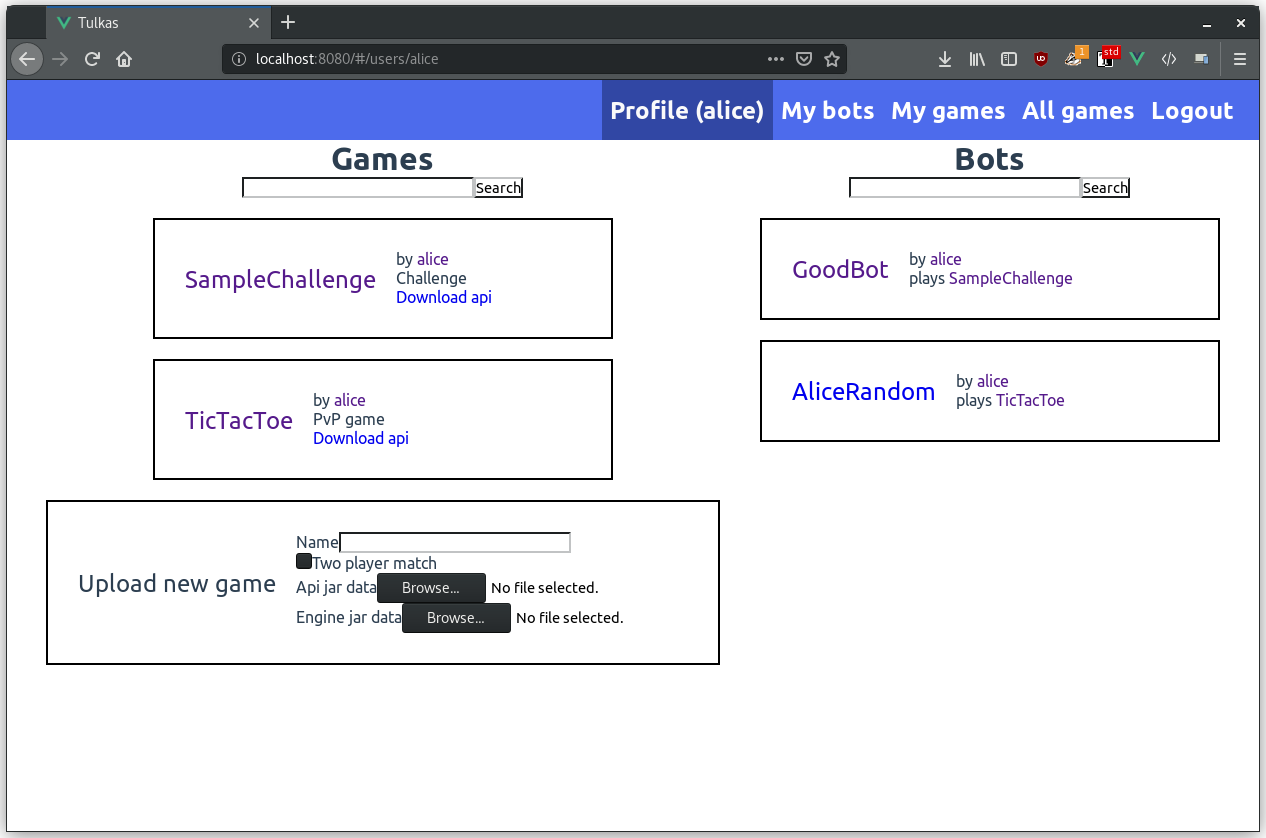
\includegraphics[width=150mm, keepaspectratio]{figures/profile.png}
		\caption*{\emph{Web interface user profile screen}} 
	\end{figure}
	\vfill

	\begin{figure}[!ht]
		\centering
		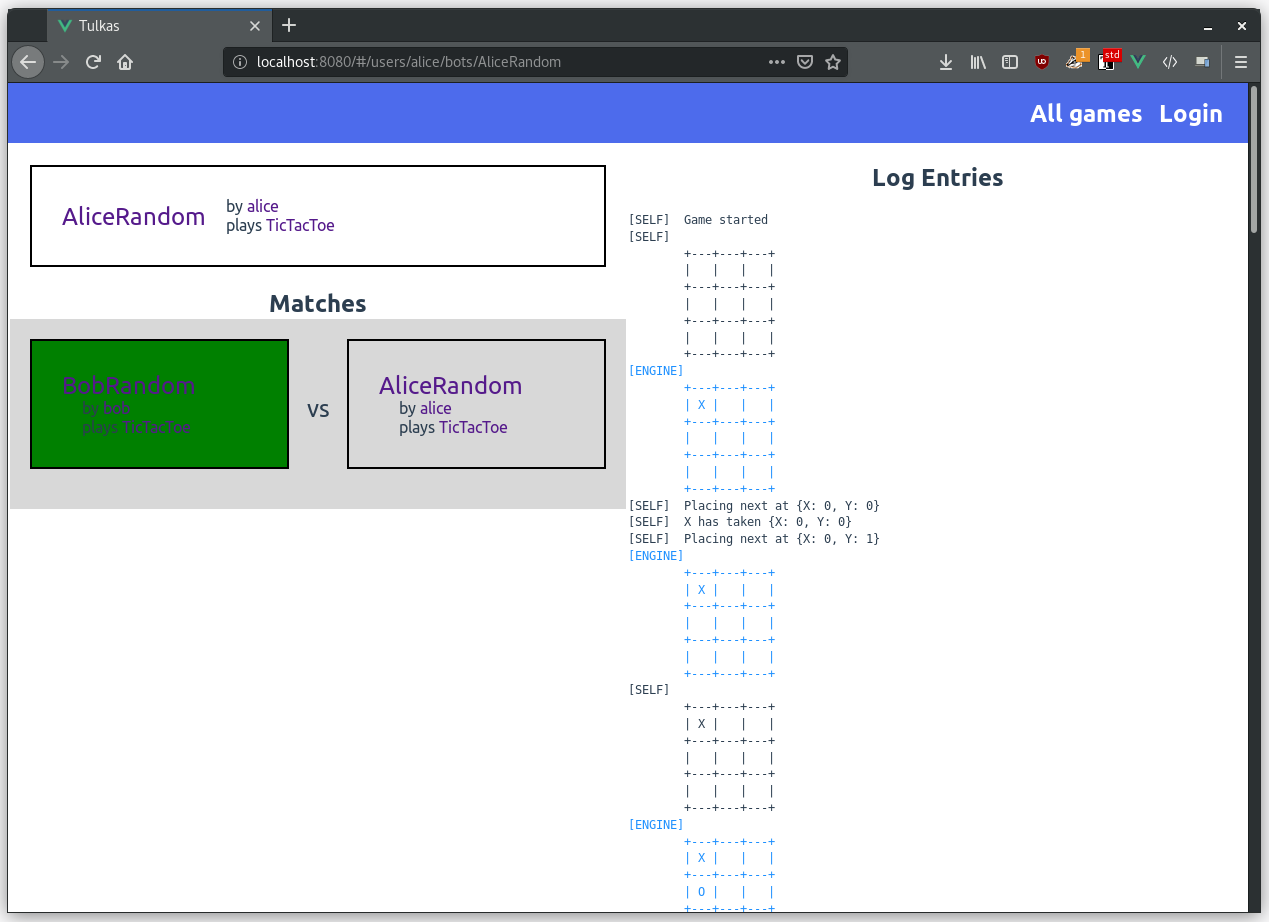
\includegraphics[width=150mm, keepaspectratio]{figures/match-log.png}
		\caption*{\emph{Web interface bot screen} \\ \emph{Played matches and log entries for selected match}} 
	\end{figure}

%\end{document}













